\documentclass[tikz,border=10pt]{standalone}
\usetikzlibrary{calc}

\begin{document}
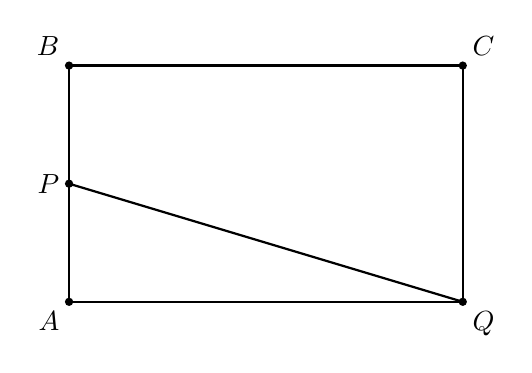
\begin{tikzpicture}
    % --- 参数定义 ---
    \def\width{5}   % 矩形宽度
    \def\height{3}  % 矩形高度
    \def\pheight{1.5} % P点距离A的高度

    % --- 定义关键点 ---
    \coordinate (A) at (0,0);
    \coordinate (B) at (0,\height);
    \coordinate (C) at (\width,\height);
    \coordinate (Q) at (\width,0);
    \coordinate (P) at (0,\pheight);

    % --- 绘制几何图形 ---
    % 绘制矩形框架
    \draw[thick] (A) -- (B) -- (C) -- (Q) -- cycle;
    
    % 绘制线段 PQ
    \draw[thick] (P) -- (Q);

    % --- 标注点 ---
    % 使用 fill 绘制实心圆点
    \foreach \point in {A,B,C,P,Q}
        \fill (\point) circle (1.5pt);

    % 标注文字
    \node[below left]  at (A) {$A$};
    \node[above left]  at (B) {$B$};
    \node[above right] at (C) {$C$};
    \node[left]        at (P) {$P$};
    \node[below right] at (Q) {$Q$};

\end{tikzpicture}
\end{document}